\chapter{\projName (think of a name for the system)} \label{chap:system}

In this chapter I would present the majority of the work we have done.
From a design perspective, implementation, and evaluation.

\section{Building Blocks}

For each one, present:
\begin{itemize}
    \item A bit of the theory behind it
    \item A basic proof of concept (maybe even bash scripts)
    \item Integration with \texttt{runc} and our system (yet to be named)
    \item A micro-benchmark of this feature.
\end{itemize}

This first section introduces the key building blocks of that make up \projName.
For each one of them we cover the theoretical concepts, the problem they try to solve, their implementation (and integration with \criu and \runc if existent), together with a targeted benchmark.

\cs{Describe the evaluation setting, versions etc.}

\cs{Link to the github repo with the benchmarking}

\subsection{Diskless Migration}

As previously detailed, \criu builds the snapshot of a running process using image (\texttt{.img}) files, which are stored in a user-specified path.
As a consequence, it relies heavily on the underlying storage facility provided which, in most commodity PCs, tends to be the disk-backed file system.
It is of no surprise then, that reading and writing from and to disk can quickly become the bottleneck in live migration performance.
It gets even worse when writes are duplicated, \textit{i.e.} we write once to disk to dump the process state, and a second time to transfer image files wherever they need to be restored.
To overcome the former, we rely on \texttt{tmpfs} a virtual memory filesystem~\cite{tmpfs-manpage}.
For the latter, we leverage \criu's \texttt{page-server}.

% TMPFS
First presented by Sun Microsystems in 2007~\cite{Snyder2007}, \texttt{tmpfs} is a memory-based file system that uses resources from the virtual memory subsystem.
According to the Linux Programmer's Manual~\cite{tmpfs-manpage}, this file system can employ swap space if memory pressure is high, only consumes as much memory as required to store the current files (regardless of the allocated size), and unmounting it destroys the contents therein.
Since the files actually reside in memory, the user benefits from memory-like read/write performance.
A notable use of \texttt{tmpfs} is \texttt{/dev/shm}, used in the POSIX-compliant implementation of shared memory and in POSIX semaphores.
One such file system can be easily created and destroyed using \texttt{mount} and \texttt{umount} as detailed in Listing~\ref{code:tmpfs-example}
\begin{lstlisting}[style=Bash,caption={Mounting and dismounting a \texttt{tmpfs} filesystem.\label{code:tmpfs-example}}]
#!/bin/bash
# Mount a tmpfs filesystem rooted in the /tmp/my-tmpfs directory with maximum size 100 MB
mkdir /tmp/my-tmpfs
sudo mount -t tmpfs -o size=100M tmpfs /tmp/my-tmpfs

# Check the new file system appears in the list of mounted devices
sudo mount | grep /tmp/my-tmpfs

# Unmount the filesystem 
sudo umount /tmp/my-tmpfs # CAUTION: THIS WILL DESTROY THE CONTENTS
\end{lstlisting}

% Page-server
The page server is a component of \criu that allows to send memory dumps directly through the network, saving disk read/writes on the origin, writing them once they reach the destination system~\cite{criu-page-server}.
Note that the page server is used only to migrate memory files, which tend to be the largest ones, whereas other image files still need to be transferred when migrating.
The current implementation uses only TCP sockets and no encryption nor compression is used on the network transfer.
It is also worth mentioning that \texttt{criu page-server --port} is a one-shot command, \textit{i.e.} if we perform multiple dumps, a page server must be started for each one of them.
Observe that, even though it introduces a small overhead, our results (see Figure~\ref{fig:diskless-migration-microbenchmark}) show that for migrations within the same machine, setting up a page server in $\texttt{localhost}$ outperforms the double-copying approach for larger applications.

% Integration w/ runC
As introduced in the previous paragraphs, the key pieces to achieve efficient diskless migrations are making use of a \texttt{tmpfs} file system and \criu's page server.
The former is in another level of abstraction than \runc, and for the latter we need to start the page server separately and then checkpoint passing address and port as a parameter to the \texttt{--page-server} flag.
In Listings~\ref{code:microbenchmark-diskless-runc} and~\ref{code:microbenchmark-diskless-criu} we include snippets to perform a checkpoint with a page server using \runc and \criu respectively.
\begin{figure}[h!]
\begin{minipage}{.45\textwidth}
\begin{lstlisting}[style=Bash,caption={Commands to perform a checkpoint in \runc using a page server.\label{code:microbenchmark-diskless-runc}}]
#!/bin/bash
# Start the Page Server
sudo criu page-server \
    --port 9999 \
    --images-dir /path/to/dst/images &

# Checkpoint using the page-server
sudo runc checkpoint \
    --image-path /path/to/src/images \
    --page-server 127.0.0.1:9999 \
    <container_name>

# To finish the migration we would need to
# copy the remaining files
# This should be fast as memory dumps are 
# already at destination
cp /path/to/src/images/* \
    /path/to/dst/images/
\end{lstlisting}
\end{minipage}\hfill
\begin{minipage}{.45\textwidth}
\begin{lstlisting}[style=Bash,caption={Commands to perfrom a checkpoint in \criu using a page server.\label{code:microbenchmark-diskless-criu}}]
#!/bin/bash
# Start the Page Server
sudo criu page-server \
    --port 9999 \
    --images-dir /path/to/dst/images &

# Checkpoint using the page-server
sudo runc checkpoint \
    --image-path /path/to/src/images \
    --page-server 127.0.0.1:9999 \
    <container_name>

# To finish the migration we would need to
# copy the remaining files
# This should be fast as memory dumps are
# already at destination
cp /path/to/src/images/* \
    /path/to/dst/images/
\end{lstlisting}
\end{minipage}
\end{figure}

% Experiment
In order to benchmark the performance of diskless migration when compared to disk-based one and the beneffits of using a page server, we set up two different experiments.
In one hand we have a counter program written in C (see Listing~\ref{code:c-counter} for the full implementation) that increments a value and prints it to \texttt{stdout}.
On the other hand we have an instance of a \redis in-memory database that we pre-load with $1e7$ keys.
The total weight of the memory image dump is $912$ MB.
For each experiment, we measure the time to checkpoint the process and transfer the remaining images to a different directory, either locally or on a different machine in the same local network.
We compare the performance when using \texttt{tmpfs} directories to store the images (diskless) or not (file-based) and when using a page server or not.
Each test is run 100 times and we present the average and standard deviation values obtained in Figure~\ref{fig:diskless-migration-microbenchmark}.

% Results
\begin{figure}[h!]
    \centering
    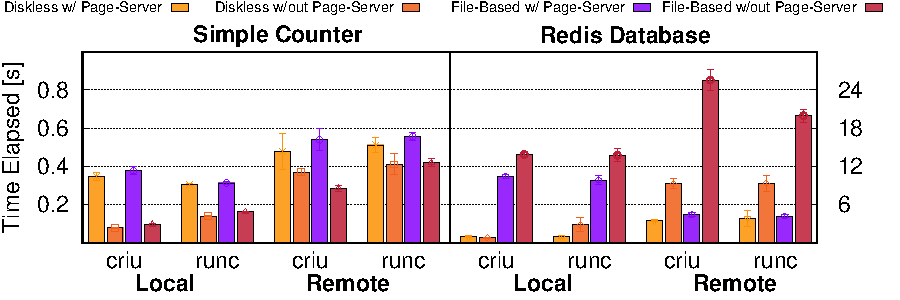
\includegraphics[width=.8\textwidth]{figs/diskless-migration-microbenchmark/diskless_migration_microbenchmark.pdf}
    \caption[Size of the memory image for iterative dumps.]{Time elapsed checkpointing and migrating a running process when using file-based or diskless migration, with and without a page server. We compare the results for a small application (around 100 kB, left) and a big one (around 1 GB, right).\label{fig:diskless-migration-microbenchmark}}.
\end{figure}

The first and most important conclusion we draw from our results is that there is no one-size-fits-all solution when choosing the best setting to migrate our application.
It seems clear that diskless is always equal or better than non-diskless.
This was to be expected, as for the same setting, \texttt{tmpfs} gives better raw read/write performance.
For instance, when transferring image files from one machine to the other, the perceived end-to-end throughput between \texttt{tmpfs} directories is in the order of 100-120 Mbps compared to the 60-70 Mbps for regular directories.
However, there might be situations, or systems, which simply don't have that much free memory.
The Redis dump files alone already take up 1 GB of memory, unacceptable in constrained devices.

If the application is sufficiently small (a dump for an instance of the counter process is around 90 kB), the overhead of running a page server is higher than simply writing the files twice, both in the local and remote setting.
However, for large applications, diskless outweighs the page server in the local case, whereas if we have to send files over the network, running a page server is more important than using the diskless approach (although a combination of both yields the best performance).
We include the full evaluation scripts in Listing~\ref{code:microbenchmark-diskless-evaluation}.

\subsection{Iterative Migration}

% Brief Introduction
%As introduced in \S

Implemented in \criu we find a series of features that enable us to perform iterative migrations of running processes.
This is, periodically snapshot the state of the process without altering it until some condition is triggered, that in turn checkpoints the container and restores it elsewhere.
The key idea being that all the heavy work for the snapshot (\textit{i.e.} capturing the memory state and transferring it) will have already been done in previous iterations, hence minimizing the application downtime.

In the previous paragraph we have assumed that transfers across consequent snapshots will be smaller in size, otherwise the $n$-th dump would not be any faster than the first one, and we would be wasting a lot of bandwidth since the same information would be sent repeatedly.
This reduction in size can be achieved through memory tracking, a procedure through which memory pages written between dumps are marked as \emph{dirty} and hence included in the following transfer.
Therefore, to implement efficient iterative migration we need:
\begin{enumerate}
    \item \textbf{Pre-Dump:} A procedure to snapshot the memory of the process without stopping it (note that, at this point, we don't need all the other details).
    \item \textbf{Memory Tracking:} A procedure to keep track of the memory changes in a process' address space.
    \item \textbf{Parent Directory:} A procedure to link together subsequent dumps so that they can be correctly re-interpreted at restore time.
\end{enumerate}

The first step during an iterative migration consists on dumping \emph{all} of the process memory to an image file.
This allows for a baseline from which smaller \emph{incremental} dumps are performed.
Note that, at this point, we are not interested in capturing the whole state, hence the usage of the \texttt{pre-dump} command in CRIU.

Memory tracking in CRIU~\cite{criu-memory-tracking} is done by means of a kernel functionality introduced in 2013~\cite{criu-memory-tracking-lwn}.
It consists of two steps: first we ask the kernel to keep track of memory changes on a per-process basis by writing a $4$ to \texttt{/proc/\$pid/clear\_refs} and, after a while, reading the \texttt{/proc/\$pid/pagemap} file and checking the \textit{soft-dirty} bit for each page table entry (PTE).
Internally, in the first step the kernel clears all soft-dirty bits \emph{and} the writable ones per each PTE for the given process id (PID).
Subsequent writes to any page will trigger a page fault, a call to \texttt{pte\_mkdirty}, and therefore the \textit{soft-dirty} bit will be set.
During the second step, at memory dump time, if this bit has not been set, the memory page needs not to be transferred again.
To enable this functionality in \criu, we must use the \texttt{--track-mem} flag.

One last key step required to achieve efficiency and correctness upon restore is to link the actual dump (or pre-dump) with the one preceding it, it's \emph{parent}.
For a pre-dump, \texttt{--prev-images-dir} indicates \criu to look for exsiting dumps in the specified path, and perform the bit-checking described in the previous paragraphs.
Upon restore, links among successive dumps are pieced together to successfully restore the freshest version of the running program.

The integration with \runc is seamless.
The pre-dump functionality is triggered with the \texttt{--pre-dump} flag which, in turn, sets the memory tracking flag automatically~\cite{runc-memtrack}.
Lastly, the \texttt{--parent-path} flag can be used to achieve the correct linkage between dumps.
In Listings \ref{code:microbenchmark-iterative-criu} and \ref{code:microbenchmark-iterative-runc} we include the different scripts to perform the three consecutive dumps both in \criu and \runc.
The complete scripts used for the benchmarking are included in Listing \ref{code:microbenchmark-iterative-evaluation}.
\begin{figure}[h!]
\begin{minipage}{.45\textwidth}
\begin{lstlisting}[style=Bash,caption={Scripts to perfrom two pre-dumps and a dump of a running process using CRIU.\label{code:microbenchmark-iterative-runc}}]
#!/bin/bash
# First Pre-Dump
sudo runc checkpoint \
    --pre-dump \
    --image-path ./images/1/ \
    <container_name>

sudo runc list # Container running

# Second Pre-Dump
sudo runc checkpoint \
    --pre-dump \
    --parent-path ../1/ \
    --image-path ./images/2/ \
    <container_name>

sudo runc list # Still running

# Last Dump
sudo runc checkpoint \
    --parent-path ../2/ \
    --image-path ./images/3/ \
    <container_name>

# Container is now stopped
\end{lstlisting}
\end{minipage}\hfill
\begin{minipage}{.45\textwidth}
\begin{lstlisting}[style=Bash,caption={Scripts to perfrom two pre-dumps and a dump of a running container using runC.\label{code:microbenchmark-iterative-criu}}]
#!/bin/bash
# First Pre-Dump
sudo criu pre-dump \
    -t  PROCESS_PID \
    --images-dir images/1 \
    --track-mem \
    --shell-job 

# Second Pre-Dump
sudo criu pre-dump \
    -t PROCESS_PID \
    --shell-job \
    --images-dir images/2 \
    --prev-images-dir ../1 \
    --track-mem

# Last Dump
sudo criu dump \
    -t  PROCESS_PID \
    --images-dir images/3 \
    --prev-images-dir ../2 \
    --shell-job \
    --track-mem

# Process is now stopped
\end{lstlisting}
\end{minipage}
\end{figure}

In order to perform a micro-benchmark of this functionality we consider two different scenarios: a simple counter written in \texttt{C}, and a \redis in-memory database, as introduced in the previous section.
For each scenario we perform two pre-dumps, and a final dump, and report the size of the \texttt{pages-1.img} file (which contains the memory dump).
We test a static setting in which we don't change the memory during successive dumps which acts as a baseline, and a dynamic one in which, between each dump, we modify the contents of the process memory.
For the counter, the static setting starts the program and goes to sleep, whereas the dynamic one indeed updates the counter every other second.
For the database, we initially pre-load it with $1e7$ key-value pairs (around 300 MB of data) and then either do nothing, or run a \texttt{redis-benchmark} which alters around $1\%$ of the key pairs.
Lastly, we compare the results of running the experiments with vanilla \criu or through \runc.

\begin{figure}[h!]
    \centering
    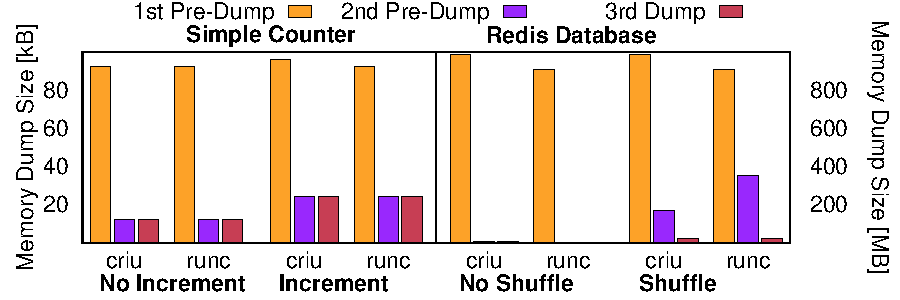
\includegraphics[width=.8\textwidth]{figs/iterative-migration-microbenchmark/iterative_migration_microbenchmark.pdf}
    \caption[Size of the memory image for iterative dumps.]{Size of the dumped memory image when performing iterative dumps. For the counter experiment we report the results in kB (left axis) and for the redis one we report the results in MB (right axis). We compare the results when using \runc or purely \criu.\label{fig:iterative-migration-microbenchmark}}.
\end{figure}

We present our results in Figure~\ref{fig:iterative-migration-microbenchmark}.
First of all, note how we use different scales for the counter application (left) and the \redis one (right).
We observe that, as expected, if we make no changes to the process' memory after the first dump, the amount of information to be re-transferred is very little, which we attribute it to \criu's metadata.
In the counter case, the initial dump is around 90 kB and subsequent ones are 12 kB, whereas in the \redis one, the size decreases from 900 MB to just 1 MB.
Once we modify the memory, additional pages need to be transferred.
In the counter case, between successive dumps we just increase the value of a variable and alter the state of \texttt{stdout}, what translates in a 10 kB inrease in the image size every time.
In the \redis one, the \texttt{redis-benchmark} is non-deterministic in nature, but it's worth observing how shuffling a percent of the total key-store propagates to higher percentages of memory re-use.
We conclude that memory tracking is a necessary feature if any application considers even near-live migration of production applications, and the technology presented allows for an easy way to do-so.


\subsubsection*{Aside: Memory Deduplication}

Maybe not an aside, but putting it here to remember

\cs{Mention that before we were optimizing a-priori, wheras this technique is a-posteriori.}

\subsection{Remote Migration}

\subsection{Checkpointing TCP Connections}

The ability to checkpoint established TCP connection is mainly due to the inclusion of the \texttt{TCP\_REPAIR} socket option to kernel version $3.5$~\cite{tcp-connection-repair}.

Similarly to other resources and as introduced in \S\ref{chap:background}, basic information about sockets is obtained by parsing the adequate files in the \texttt{/proc} filesystem.
However, there are some internals of active network connections (namely negotiatied parameters such as send and receive queues, and sequence numbers) that require putting the socket in the \texttt{TCP\_REPAIR} state using the \texttt{setocketopt()} syscall (note that this action requires \texttt{CAP\_NET\_ADMIN} capabilities).
Then, if the connection is closed whilst the socket is in \texttt{TCP\_REPAIR} mode, no \texttt{FIN} nor \texttt{RST} packets are sent to the other peer, what means that his endpoint is effectively still open~\cite{Corbet12}.

To re-establish the connection from the newly generated socket, the first thing to do is put it, again, in \texttt{TCP\_REPAIR} mode.
Then, the previously dumped parameters can be set, and upon \texttt{connect()} the socket goes directly into \texttt{ESTABLISHED} mode without acknowledgment from the other end, and a \texttt{RST} packet is sent to resume communication.

% TABLE FILTERING
The last missing piece is what happens if the remote end tries to send a packet to its, seemingly open, TCP socket whilst the other peer is down.
Were we to ignore this fact, once the packet reached our kernel this, given that the socket is closed, would send a \texttt{RST} to the other end, and our whole illusion would collapse.
To overcome this issue, upon checkpoint we include a set of rules to the \texttt{netfilter}~\cite{netfilter} IP routing table to drop all packets.
We include the set of rules in Table~\ref{table:iptables-rules}.
\begin{table}[h!]
    \centering
    {\ttfamily 
    \begin{tabular}{p{3cm}p{1cm}p{1cm}p{2.5cm}p{2.5cm}p{5.0cm}}
        \multicolumn{6}{l}{Chain INPUT (policy ACCEPT)} \\[3pt]
        target & prot & opt & source & dest & \\[3pt]
        CRIU & all & -- & <source\_IP> & <dest\_IP> & \\[3pt]
        & & & & & \\[3pt]
        \multicolumn{6}{l}{Chain FORWARD (policy ACCEPT)} \\[3pt]
        target & prot & opt & source & dest & \\[3pt]
        & & & & & \\[3pt]
        \multicolumn{6}{l}{Chain OUTPUT (policy ACCEPT)} \\[3pt]
        target & prot & opt & source & dest & \\[3pt]
        CRIU & all & -- & <source\_IP> & <dest\_IP> & \\[3pt]
        & & & & & \\[3pt]
        \multicolumn{6}{l}{Chain CRIU} \\[3pt]
        target & prot & opt & source & dest & \\[3pt]
        ACCEPT & all & -- & <source\_IP> & <dest\_IP> & mark match ! 0xc114\\[3pt]
        DROP & all & -- & .../0 & .../0 & \\[3pt]
    \end{tabular}
    }
    \caption{Output of running \texttt{iptables -t filter -L -n}.\label{table:iptables-rules}}.
\end{table}

\textbf{Efficient IP Address Re-Use}

A caveat of restoring established TCP connections is that, without bringing down both peers, we can not circumvent the negotiated \texttt{IP:PORT} pairs.
As a consequence, the same IP address and port must be available at restore time.
Otherwise, when the remote peer receives the \texttt{RST} package it will immediately close the connection.
Re-using an IP address is achievable using locally scoped addresses or network namespaces.
In our experiments we tested both.

Firstly, if we are migrating into a different machine (as the experiments presented below), we need to assign addresses using \texttt{ip}'s \texttt{addr} subcommands.
In particular, we are using a \texttt{host-only}~\cite{vbox-hostonly} subnet to manage our (virtual) machines.

Alternatively, we have also tested process migration within the same machine, from one network namespace to a different one.
This situation is particularly interesting as it recreates what happens under the hood in \criu's binding for \runc, as containers rely on namespaces for isolation.
We set up a bridge device in the host namespace, two network namespaces, and two virtual ethernet devices with one peer tied to the bridge, and the other one inside a namespace.
Adequately setting up addresses and default gateway routes, we achieve the setup we depict in Figure~\ref{fig:veth-arch}.
\begin{figure}[h!]
    \centering    
    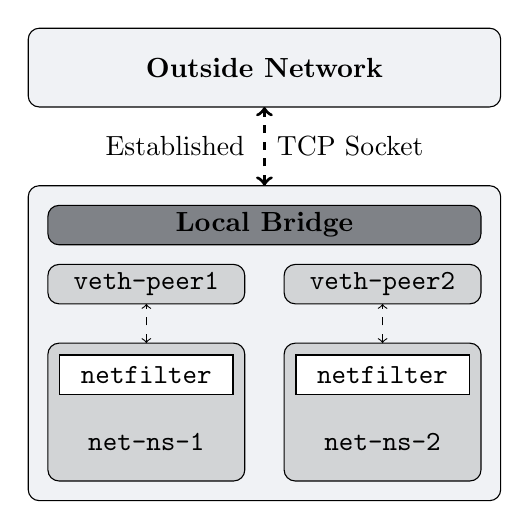
\begin{tikzpicture}
        % Color definition
        \definecolor{machineBG}{RGB}{240, 242, 245}
        \definecolor{namespaceBG}{RGB}{210, 212, 214}
        \definecolor{bridgeBG}{RGB}{127, 130, 135}

        % Host network box
        \draw[fill=machineBG, rounded corners] (0,0) rectangle (6, 4);
        % Network Namespace 1 and Peer
        \draw[fill=namespaceBG, rounded corners] (0.25, 0.25) rectangle (2.75, 2.0);
        \node at (1.5, 0.75) {\textbf{\texttt{net-ns-1}}};
        \draw[fill=white] (0.4, 1.35) rectangle (2.6, 1.85) node[pos=.5] {\text{\texttt{netfilter}}};
        \draw[<->, dashed] (1.5,2) -- (1.5,2.5);
        \draw[fill=namespaceBG, rounded corners] (0.25, 2.5) rectangle (2.75, 3) node[pos=.5] {\text{\texttt{veth-peer1}}};
        % Network Namespace 2
        \draw[fill=namespaceBG, rounded corners] (3.25, 0.25) rectangle (5.75, 2.0);
        \node at (4.5, 0.75) {\textbf{\texttt{net-ns-2}}};
        \draw[fill=white] (3.4, 1.35) rectangle (5.6, 1.85) node[pos=.5] {\text{\texttt{netfilter}}};
        \draw[<->, dashed] (4.5,2) -- (4.5,2.5);
        \draw[fill=namespaceBG, rounded corners] (3.25, 2.5) rectangle (5.75, 3) node[pos=.5] {\text{\texttt{veth-peer2}}};
        % Local Bridge
        \draw[fill=bridgeBG, rounded corners] (0.25, 3.25) rectangle (5.75, 3.75) node[pos=.5] {\textbf{Local Bridge}};

        % Connecting line
        \draw[<->, dashed, very thick] (3,4) -- (3,5) node[pos=.5] {Established \hspace{5pt} TCP Socket};

        % Outside network box
        \draw[fill=machineBG, rounded corners] (0,5) rectangle (6, 6) node[pos=.5] {\textbf{Outside Network}};
    \end{tikzpicture}
    \caption{Architecture of three different namespaces connected through virtual ethernet pairs.\label{fig:veth-arch}}
\end{figure}

Integration with \runc is two-fold.
For the TCP connection \criu's binding for \runc includes a \texttt{--tcp-established} flag that does most of the socket management.
If we are interested in restoring the connection in a different machine or namespace, we must manually recreate the filter table from Table~\ref{table:iptables-rules} using the \texttt{iptables} command.
Lastly, to restore into an existing namespace, the container must be restored with the adequate open file descriptors using \criu's \texttt{--external}~\cite{criu-external} and \texttt{--inherit-fd}~\cite{criu-inherit-fd}.
In Listings~\ref{code:microbenchmark-tcp-nonetns} and~\ref{code:microbenchmark-tcp-netns} we include excerpts of snippets to checkpoint and restore a established TCP connection without or within a network namespace respectively.
The complete scripts for the evaluation are included in Listings~\ref{code:microbenchmark-tcp-criu-downtime} and~\ref{code:microbenchmark-tcp-criu-reactivity} for \criu's downtime and reactivity experiments, and in Listings~\ref{code:microbenchmark-tcp-runc-downtime} and~\ref{code:microbenchmark-tcp-runc-reactivity} for \runc's.
\begin{figure}[h!]
\begin{minipage}{.45\textwidth}
\begin{lstlisting}[style=Bash,caption={Checkpoint and restore an established TCP connection using \criu and \runc.\label{code:microbenchmark-tcp-nonetns}}]
#!/bin/bash
# CRIU Dump and Restore, one after the other 
# but in the BG (not affecting time)
(sudo criu dump \
    -t ${SERVER_PID} \
    --images-dir ${IMAGES_DIR} \
    --tcp-established; \
echo "Restoring server..."; \
sudo criu restore \
    --images-dir ${IMAGES_DIR} \
    --tcp-established) &

# Similarly with runC
(sudo runc checkpoint \
    --image-path ${IMAGES_DIR} \
    --tcp-established \
    eureka; \
cd /container/directory; \
sudo runc restore \
    --image-path ${IMAGES_DIR} \
    --tcp-established \
    eureka; \
cd ${CWD}) &
\end{lstlisting}
\end{minipage}\hfill
\begin{minipage}{.45\textwidth}
\begin{lstlisting}[style=Bash,caption={Excerpt of a script to checkpoint a connection within an existing namespace, and inherit it on restore.\label{code:microbenchmark-tcp-netns}}]
#!/bin/bash
# Two namespaces with path NS_1 and NS_2
INO_1=$(ls -iL ${NS_1} | awk '{ print $1 }')
INO_2=$(ls -iL ${NS_2} | awk '{ print $1 }')
exec 33< ${NS_1}
exec 34< ${NS_2}

# To checkpoint we mark as an external
# resource both NS
sudo criu dump \
    -t ${PID_1} \
    --images-dir images \
    --tcp-established \
    --external net[${INO_1}]:${NS_1} \
    --external net[${INO_2}]:${NS_2}

# At restore, we match the file 
# descriptors with the NS
sudo criu restore \
    --images-dir images \
    --tcp-established \
    --inherit-fd fd[33]:${NS_1} \
    --inherit-fd fd[34]:${NS_2} -d
\end{lstlisting}
\end{minipage}
\end{figure}

\textbf{Benchmarking}

In order to evaluate the impact of migrating a process with an established TCP connection, we are interested in assessing how quickly can communication resume after restore.

To achieve this goal we set up the following testbed.
We first deploy two identical virtual machines running Linux Debian with kernel version \texttt{4.19.0-6}.
Each one has \criu version 3.13 and \runc version \texttt{1.0.0-rc8}, both built from source.
Additionally, and in order to conduct the experiments, we make use of \texttt{iPerf3} (version \texttt{3.7+}) a network bandwidth benchmarking tool~\cite{iperf3}.
In particular, we start an \texttt{iPerf3} client-server pair, one in each VM, and record the perceived throughput by the client.
Each experiment is repeated running the bare processes and checkpointing them using \criu, or isolating them within a \runc container, to assess the introduced overhead.
We measure from the client side since we are interested in dumping and restoring the server.
This situation makes more sense from the cloud-provider/load-balancing standpoint.

\textbf{Re-connection after a down period.}
The first experiment simulates the scenario in which the server is restored some time after the dump occured.
In particular, we let the client saturate the link for 10 seconds, then dump the server, and restore it 2 seconds later, all of which transparently to the client (whose connection is never closed).
In Figure~\ref{fig:evaluation-downtime} we present the throughput perceived by the client as a function of time. 
\begin{figure}[h!]
    \centering
    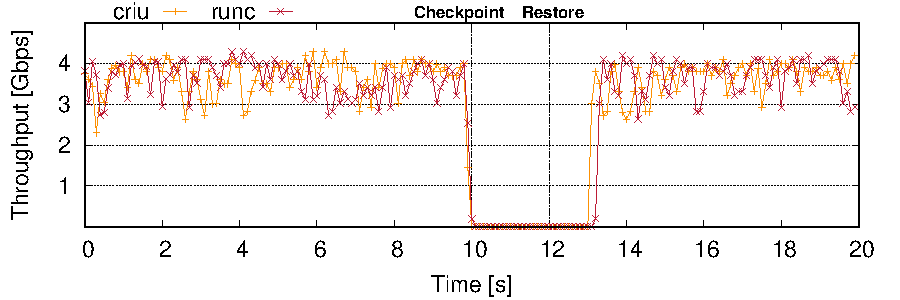
\includegraphics[width=\linewidth]{./figs/tcp-established-downtime/tcp_established_downtime_microbenchmark.pdf}
    \caption{Throughput perceived from the client as a function of time, when we checkpoint the server once, and restore it after two seconds. We compare the results of \criu and \runc. \label{fig:evaluation-downtime}}
\end{figure}
The first observation we make from the plot, is that it takes almost a full second to get the connection back to full speed.
To understand this behaviour we must recall what is \texttt{iPerf3} actually doing.
The client tries to saturate the link, sending as many packets as it can, and reports the measured capacity.
As the socket is never closed, and packets are just discarded by the network filters, to the client it will be as if those packets were never acknowledged, and hence will try to retransmit them.
The TCP protocol specifies~\cite{tcp-rfc} that the retransmission timeout must be doubled every time a packet is not acknowledged, therefore the recurrent outage of ACKs might cause the client to back-off for the perceived full second.
This implies that checkpointing established TCP connections only makes sense in the scenario in which the service is soon going to be restored.
The next experiment tackles the behaviour under this situation.

\textbf{Reactivity to immediate restore.}
To prove our hypothesis that the large delay after a restore is due to the protocol itself rather than our implementation, we set up an experiment in which we perform a sequence of dumps and immediate restores of the same established TCP connection.
We again present the throughput as a function of time in Figure~\ref{fig:evaluation-reactivity}.
\begin{figure}[h!]
    \centering
    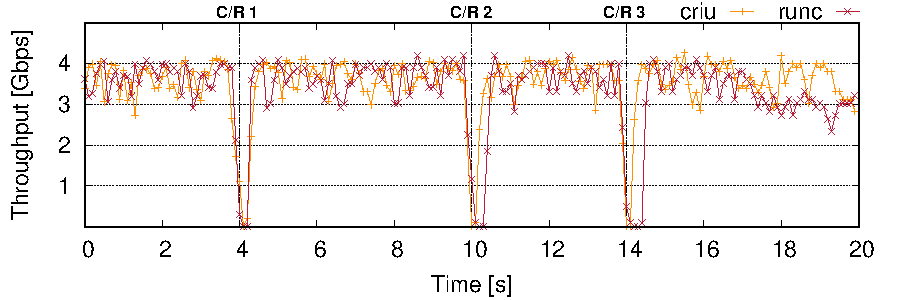
\includegraphics[width=\linewidth]{./figs/tcp-established-resolution/tcp_established_resolution_microbenchmark.pdf}
    \caption{Throughput from the client as a function of time.\label{fig:evaluation-reactivity}}
\end{figure}
In this case the measured throughput downtime does not exceed $0.1$ seconds, an order of magnitude better than the previous experiment.
This reduced value, together with the fact that the application studied is very network-intensive, makes us believe that our proposed technique is suitable for most client-server scenarios and won't have an impact in the overall quality of service.

Lastly, in both Figures we observe that, albeit being the experiments running bare processes with \criu slightly faster to restore, the overhead introduced by \runc is negligible.

\section{Checkpointing Multiple Containers}

To be done.
A necessary first step is to manage the namespaces and IPs as we do now.

\section{Putting it All Together}

A bit of a walkthrough of the final implementation
